\documentclass{curietheme} %
%\documentclass[handout]{beamer} %
\usetheme{Frankfurt}
\usepackage[latin1]{inputenc}
\usefonttheme{serif}
\usepackage{times}
\usepackage{tikz}
\usepackage{amsmath}
\usepackage{verbatim}
\usetikzlibrary{arrows,shapes,backgrounds}
\usepackage{pstricks}
\usetikzlibrary{shapes.callouts,decorations.pathmorphing}
\usepackage{wrapfig}
\usepackage{multimedia}
\definecolor{gold}{rgb}{0.85,.66,0}
\def\reff#1{(\ref{#1})}

\def\diff{\mathrm{d}}
\def\imagi{\mathrm{i}}

\def\halb{\frac{1}{2}}

\def\pabl#1#2{\frac{\partial #1}{\partial #2}}

\def\omegaone{\begin{color}{blue}\omega_1\end{color}}
\def\TcalopKS{\hat{ T}_{\mathrm{KS}}}

\def\Vcalop{\hat{ V}}

\def\Tcalop{\hat{ T}}

\def\Hintop{\hat{H}}


\def\Vopee{\hat{V}_{{ee}}}
\def\psiopdag{\hat{\psi}^{\dagger}}
\def\psiop{\hat{\psi}}
\def\vext{v_{\mathrm{ext}}}
\def\Vee{V_{ee}}
\def\vee{v_{ee}}
\def\nop{\hat{n}}
\def\Uop{\hat{U}}
\def\Vop{\hat{V}}
\def\Vintop{\hat{V}^{\mathrm{int}}}
\def\Wop{\hat{W}}
\def\bop{\hat{b}}
\def\bopdag{\hat{b}^{\dagger}}
\def\qop{\hat{q}}
\def\Eop{\hat{E}}
\def\jop{\hat{j\,}}
\def\vHxc{v_{\mathrm{Hxc}}}
\def\vHx{v_{\mathrm{Hx}}}
\def\vH{v_{\mathrm{H}}}
\def\vc{v_{\mathrm{c}}}
\def\xop{\hat{x}}
\def\Ahe{\mathcal{A}(\mathrm{white-region})}
\def\Aheplus{\mathcal{A}(\mathrm{yellow-region})}
\def\Aheplusplus{\mathcal{A}(\mathrm{blue-region})}





\def\beq{\begin{equation}}
\def\eeq{\end{equation}}

\def\beqa{\begin{eqnarray}}
\def\eeqa{\end{eqnarray}}
\def\energy{{\cal E}}
\def\energykin{{\cal E}_\mathrm{kin}}

\def\eulere{\mathrm{e}}

\def\Ehat{\hat{E}}
\def\Ahat{\hat{A}}

\def\ket#1{\vert #1\rangle}
\def\bra#1{\langle#1\vert}
\def\braket#1#2{\langle #1 \vert #2 \rangle}

\def\vekt#1{\bm{#1}}
\def\vect#1{\vekt{#1}}
\def\vektr{\vekt{r}}

\def\makered#1{{\color{red} #1}}

\def\Im{\,\mathrm{Im}\,}

\def\varphic{\varphi_{\mathrm{c}}}

\def\Up{U_\mathrm{p}}
\def\vxc{v_\mathrm{xc}}
\def\vextop{\hat{v}_\mathrm{ext}}
\def\VC{V_\mathrm{c}}
\def\VHX{V_\mathrm{Hx}}
\def\VHXC{V_\mathrm{Hxc}}
\def\wop{\hat{w}}
\def\Gammaevenodd{\Gamma^\mathrm{even,odd}}
\def\Gammaeven{\Gamma^\mathrm{even}}
\def\Gammaodd{\Gamma^\mathrm{odd}}
\def\zetabar{\bar{\zeta}}
\def\psibar{\bar{\psi}}
\def\Psibar{\bar{\Psi}}
\def\hamop{\hat{{\cal H}}}
\def\hamopKH{\hat{{\cal H}}_\mathrm{KH}}
\def\Hop{\hat{H}}
\def\Gop{\hat{G}}
\def\GKH{\hat{G}_\mathrm{KH}}
\def\Pop{\hat{P}}
\def\pop{\hat{p}}
\def\HopKS{\hat{H}_\mathrm{KS}}
\def\HKS{H_\mathrm{KS}}
\def\Top{\hat{T}}
\def\TopKS{\hat{T}_\mathrm{KS}}
\def\VopKS{\hat{V}_\mathrm{KS}}
\def\VKS{{V}_\mathrm{KS}}
\def\vKS{{v}_\mathrm{KS}}
\def\Ttildeop{\hat{\tilde{T}}}
\def\Ttilde{{\tilde{T}}}
\def\Vextop{\hat{V}_{\mathrm{ext}}}
\def\Vext{V_{\mathrm{ext}}}
\def\Vopee{\hat{V}_{{ee}}}
\def\psiopdag{\hat{\psi}^{\dagger}}
\def\psiop{\hat{\psi}}
\def\vext{v_{\mathrm{ext}}}
\def\Vee{V_{ee}}
\def\vee{v_{ee}}
\def\nop{\hat{n}}
\def\Uop{\hat{U}}
\def\Wop{\hat{W}}
\def\bop{\hat{b}}
\def\bopdag{\hat{b}^{\dagger}}
\def\qop{\hat{q}}
\def\jop{\hat{j\,}}
\def\vHxc{v_{\mathrm{Hxc}}}
\def\vHx{v_{\mathrm{Hx}}}
\def\vH{v_{\mathrm{H}}}
\def\vc{v_{\mathrm{c}}}
\def\xop{\hat{x}}
\def\hop{\hat{h}}
\def\varphiexact{\varphi_{\mathrm{exact}}}
\def\xvec{\textbf{x}}
\def\rvec{\textbf{r}}
\def\pvec{\textbf{p}}
\def\Avec{\begin{color}{red}\textbf{A}\end{color}}
\def\Evec{\textbf{E}}

\def\fmathbox#1{\fbox{$\displaystyle #1$}}

\usepackage{tikz,graphicx}
\usetikzlibrary{decorations.markings}

\definecolor{myyellow}{RGB}{254,241,24}
\definecolor{myorange}{RGB}{234,125,1}


\title{Filament tracking to cell force measurements:
\bigskip\newline
\small{ Gaussian polynomial models, gradient descent, random forest classifier}}

\author{\underline{Varun Kapoor}}

\institute{Institute Curie, Paris}


\date{March 16, 2018}

\begin{document}

\tikzstyle{every picture}+=[remember picture]

\tikzstyle{na} = [baseline=-0.6ex]
\begin{frame}
% Cover slide
\titlepage 

\end{frame}

\begin{frame}
  \frametitle{Outline}

  \tableofcontents
  % You might wish to add the option [pausesections]
\end{frame}



\section{Motivation}

\frame{\frametitle{Motivation}
\begin{center}
\includegraphics[clip=true,width=0.5\textwidth]{Fig1AMT.png}
\end{center}

 
\begin{block}{}
\begin{itemize}
\item Computer Vision/ Machine Learning algorithms $\rightarrow$ enables object recognition (MT).
\item Cylindrical Protein Polymers $\rightarrow$ Gaussian Polynomials do the localization.
\end{itemize}
\end{block}



%\begin{tikzpicture}[overlay]
 %       \path[->]<1-> (n1) edge [] (t1);
     
      
%\end{tikzpicture}
%\item Exact time-dependent xc potentials are an unknown in TDDFT.  Exact constructions can lead to better approximations or show limitations of TDDFT.
%\end{itemize}

%\begin{itemize}
%\item Effort to propagate time-dependent $N$-body wavefunction scales exponentially with the particle number $N$; prohibitive for $N> 2$ (``exponential wall'').\pause
%\item Time-dependent density functional theory (TDDFT) is a density-based method to obtain time-dependent quantum dynamics of a many-body system; scales (almost) linearly with $N$.\pause	
%\item Time-dependent exchange-correlation (xc) potentials in TDDFT contain (in principle) all the time-dependent many-body correlation effects.\pause
%\item Exact time-dependent xc potentials are an unknown in TDDFT.\pause \; Exact constructions can lead to better approximations or show limitations of TDDFT.
%\end{itemize}

%\end{center}
}







\frame{\frametitle{Trajectory Analysis}
\begin{center}  
\includegraphics[clip=true,width=0.45\textwidth]{Fig4MT.png}

\end{center}

\begin{block}{}

Problem part B: Automate rates and statistics.

\end{block}
}


%\begin{frame}



%\tikz[baseline]{
 %           \node[fill=green!30,ellipse,anchor=base,fill opacity=0.5] (t3)
  %          {Describing autoionization in TDDFT with single orbital.};
   %     }
      
   
%\tikz[baseline]{
 %           \node[fill=purple!30,ellipse,anchor=base,fill opacity=0.5] (t4)
  %          {Adiabatic TDDFT potentials miss these states.};
   %     }     
        

%\tikz[baseline]{
 %           \node[fill=blue!30,ellipse,anchor=base,fill opacity=0.5] (t5)
  %          {Exact orbitals and potentials must be computed.};
   %     }     
        

\section{Gaussian Polynomial Models }
\subsection{Tracking FIlaments at Sub-pixel accuracy}



\frame{

\begin{center}\Huge
Part 1 


\medskip
Locating and Localizing MT
$$\downarrow$$ 
``Computer Vision and Mathematics''

\end{center}

}





\frame{\frametitle{Locate and Localize}

\begin{center}
\includegraphics[clip=true,width=0.7\textwidth]{Fig2AMT.png}
\end{center}



}

\frame{\frametitle{Error Stats}

\begin{center}
\includegraphics[clip=true,width=0.7\textwidth]{Fig2BMT.png}
\end{center}



}

\frame{\frametitle{Gaussian Line Model}



\begin{center}
\tikz[baseline]{
            \node[fill=cyan!150, ellipse,anchor=base] (t1){ 
Localizing End points of MT seeds:};}

\bigskip

\bigskip

We developed Gaussian Line model as sum of Gaussians along a line

\bigskip
$\downarrow$
\bigskip

$G(x,y)\delta(y - m  x - c)$

\bigskip
$\downarrow$
\bigskip

$G(x_i,y_i) = A\sum_i \exp{\left[- \left(\frac{x-x_i}{\sigma_x}\right)^2 - \left(\frac{y-y_i}{\sigma_y}\right)^2  \right] } + B$

\bigskip
$\downarrow$
\bigskip

Parameters of the model $\vec{\theta} = (A, B, (x_s, y_s), (x_e, y_e), \vec{ds} = (dx, dy))$.


\end{center}

}

\frame{\frametitle{Optimization}
\begin{itemize}

\item Using the model minimize $\chi^2 = \sum_{\mathrm{pixels}}[ I_{ij} - F(\vec{x}, \vec{\theta}) ]^2$. 
\item $I_{ij} $ is Image intensity at $\vec{x}$.\pause

\end{itemize}


\begin{center}
\tikz[baseline]{
            \node[fill=cyan!150, rectangle,anchor=base] (t1){ 
Minimization is done using Levenberg-Marquardt solver};}

\bigskip
$\downarrow$
\bigskip

Improve answer by doing weighted centre of mass fit using N Gaussians

\bigskip
$\downarrow$
\bigskip

$(x_c, y_c) = \frac{\sum_{ij}X_{ij}I_{ij}W_{ij}}{\sum_{ij}I_{ij}}$

\bigskip

$W_{end}(x,y) = \sum_i\exp\left[  -\left(\frac{\vec{x} + \vec{ds}_i - \vec{x}_c}{\vec{\sigma}}\right)^2  \right] $
$W_{start}(x,y) = \sum_i \exp\left[  -\left(\frac{\vec{x} - \vec{ds}_i - \vec{x}_c}{\vec{\sigma}}\right)^2  \right] $
\end{center}

}

\frame{\frametitle{Real Examples}


\begin{center}
\begin{columns}  

 \begin{column}{0.33\textwidth} 
MSER
\includegraphics[clip=true,width=0.91\textwidth]{Seed_example.png}
\newline
\includegraphics[clip=true,width=0.91\textwidth]{Seed_example2.png}
\end{column}

 \begin{column}{0.33\textwidth} 
 MSER
\includegraphics[clip=true,width=1\textwidth]{Mserexample.png}
\newline
\includegraphics[clip=true,width=1\textwidth]{MserexampleSeed.png}
\end{column}

 \begin{column}{0.33\textwidth} 
 Watershed + Hough
 \includegraphics[clip=true,width=1\textwidth]{Watershedimage.jpg}
\newline
\includegraphics[clip=true,width=1\textwidth]{HoughSeedexample.png}
\end{column}


\end{columns}
\end{center} 
}


\frame{

\begin{center}\Large
Location and Localization (t)



\end{center}
}


\frame{\frametitle{From biology to mathematics}



\begin{itemize}

\item MTs are cylindrical polymers, as an Image appear as Gaussian Polynomials.

\bigskip
\begin{columns}  

 \begin{column}{0.5\textwidth} 

{\includegraphics[clip=true,width=1\textwidth]{MThigh.png}}

\end{column}

 \begin{column}{0.5\textwidth} 



\item Now we need to upgrade the Line model to a Polynomial model
\item $G(x,y)\delta(y - d x^3 - e x^2 - m  x - c)$

\end{column}
\end{columns}


\end{itemize}




}


\frame{\frametitle{The polynomial Models}



\begin{center}

\tikz[baseline]{
            \node[fill=cyan!150, ellipse,anchor=base] (t1){ 
Localization in time};}

\bigskip



\bigskip
$\downarrow$
\bigskip

$G(x,y)\delta(y - d x^3 -e x^2 - m  x - c)$

\bigskip
$\downarrow$
\bigskip

$G(x_i,y_i) = A\sum_i \exp{\left[- \left(\frac{x-x_i}{\sigma_x}\right)^2 - \left(\frac{y-y_i}{\sigma_y}\right)^2  \right] } + B$

\bigskip
$\downarrow$
\bigskip

Parameters of the model $\vec{\theta} = (A, B, (x_s, y_s), (x_e, y_e), \vec{ds} = (dx, dy), d, e)$.


\end{center}



}






\frame{\frametitle{Real-Time tracking}


\begin{center}
\movie[width=1\textwidth, height= 0.5\textwidth]{Click}{smalltest.avi}
\end{center}
}

\frame{\frametitle{Ransac Fits}


\begin{itemize}

\item RANSAC is a technique to find outliers in data: \\ Iterative regression using a function.




\end{itemize}


\begin{center}

\tikz[baseline]{
            \node[fill=cyan!150, ellipse,anchor=base] (t1){ 
RANSAC on a Random walker};}

\bigskip



\bigskip
$\downarrow$
\bigskip


Random Walk trajectories appear like polynomials (zig-zag curves).


\bigskip
$\downarrow$
\bigskip


We use second/ third order regularized polynomial to find inliers.

\bigskip
$\downarrow$
\bigskip

On those inliers we fit a line to determine rates (min 3 time-points).

\end{center}



}

\frame{\frametitle{Ransac Fits}

\begin{center}
{\includegraphics[clip=true,width=0.45\textwidth]{Fig4MT.png}}\\
\end{center}
}



\frame{

\begin{center}\Huge
Part 2


\medskip
Ellipse Fitting to determine embryonic forces

\end{center}

}


\section{Ellipse fitting using Ransac}
\subsection{Using Random Forest Classifier for full automation}

\frame{\frametitle{}



\begin{columns}
 \begin{column}{0.5\textwidth} 
{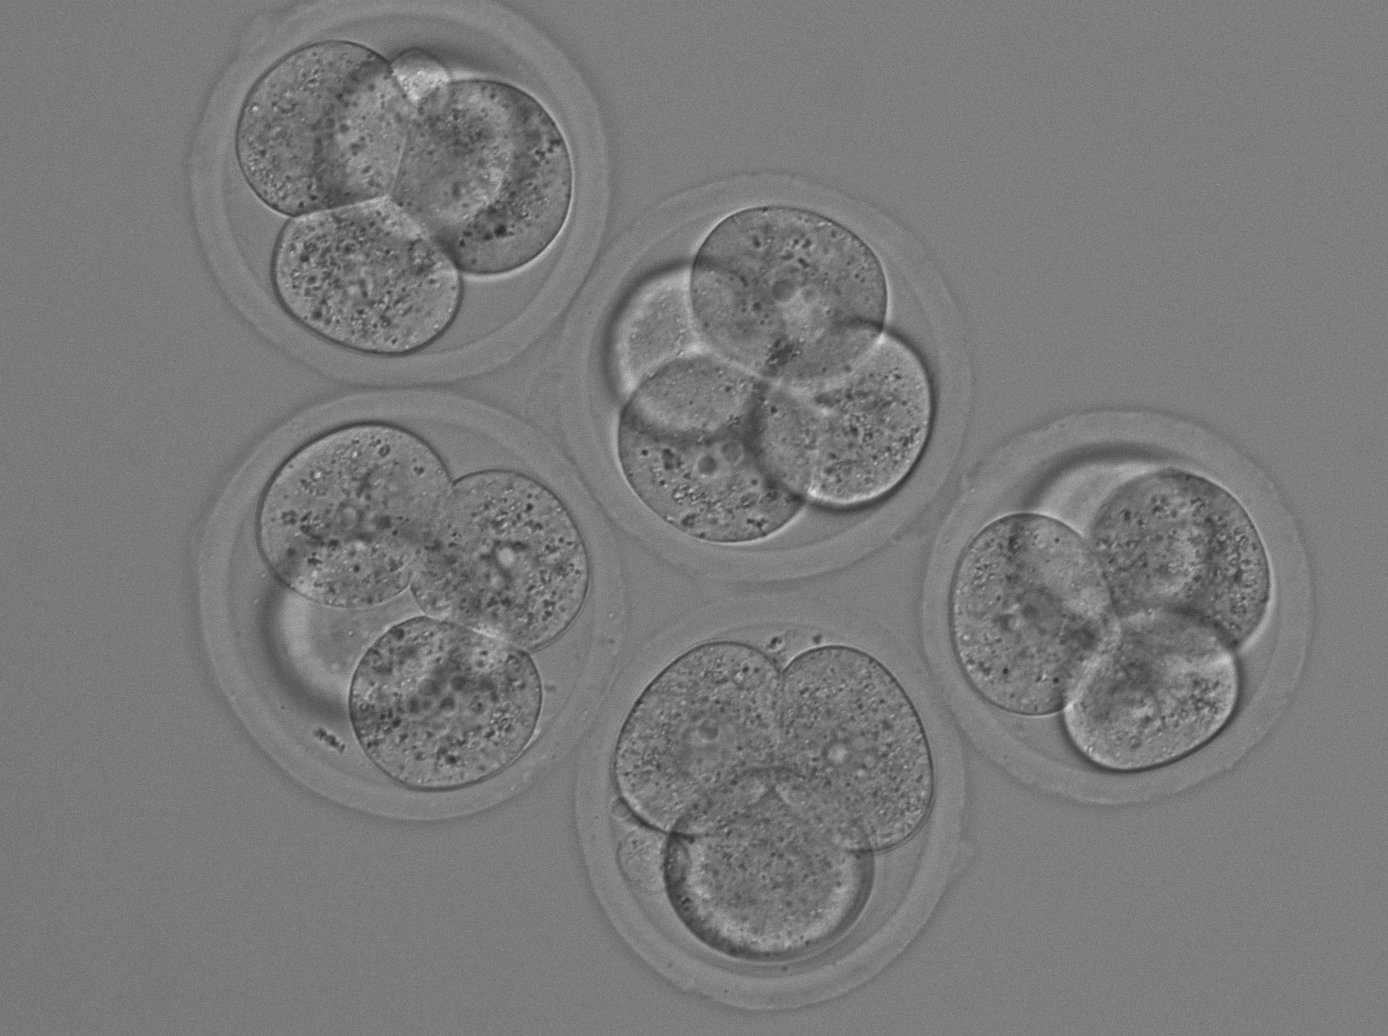
\includegraphics[clip=true,width=1\textwidth]{EmbryoA.jpg}}\\
\end{column}
 \begin{column}{0.5\textwidth} 
{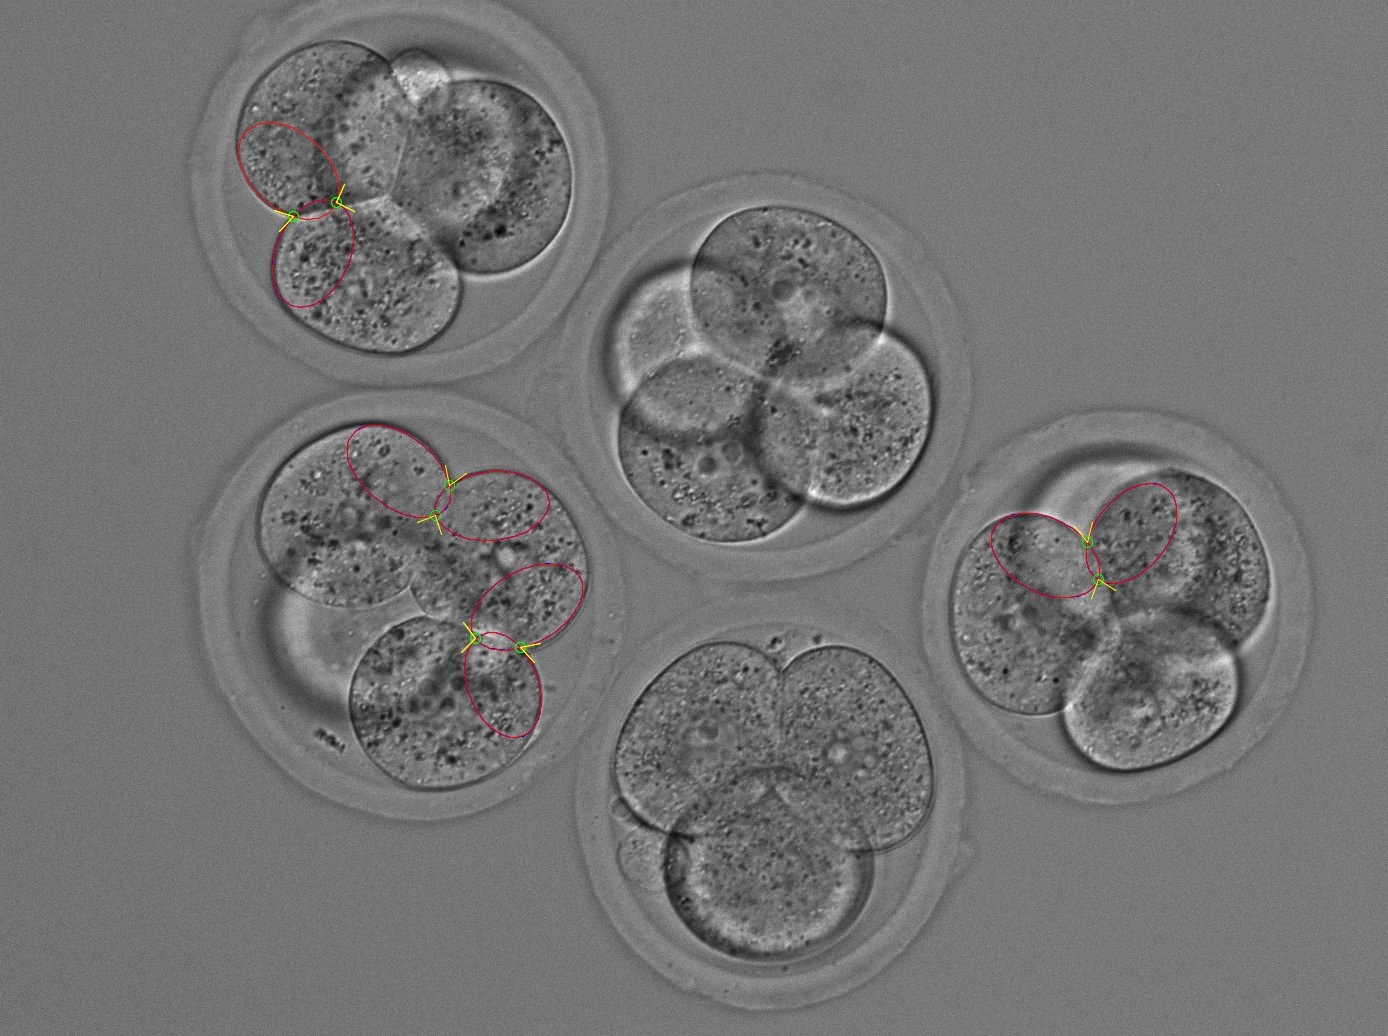
\includegraphics[clip=true,width=1\textwidth]{EmbryoB.jpg}}\\
\end{column}
\end{columns}


}

\frame{\frametitle{Ransac for 3D ellipsoid fitting}

\begin{center}
{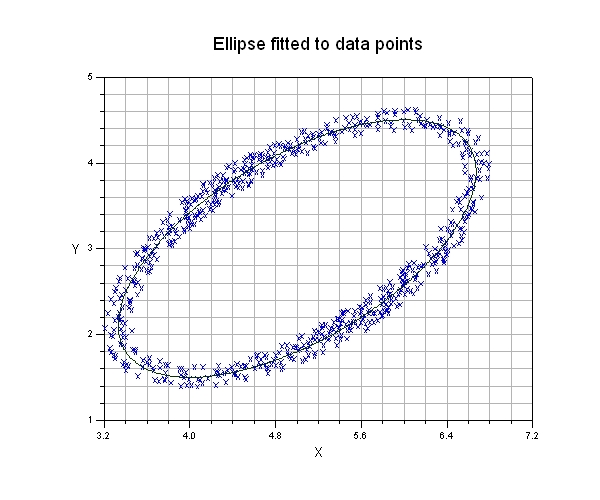
\includegraphics[clip=true,width=0.45\textwidth]{ellipsefitexample.jpg}}\\
\end{center}
\begin{itemize}
\item Require closest distance of a point from the ellipsoid. \href{https://github.com/kapoorlab/imglib2-algorithm/blob/master/src/main/java/net/imglib2/algorithm/ransac/RansacModels/DistPointHyperEllipsoid.java}{Code here}
\item Regression based ellipse fit on the inliers. \href{https://github.com/kapoorlab/imglib2-algorithm/blob/master/src/main/java/net/imglib2/algorithm/ransac/RansacModels/FitEllipsoid.java}{Code here}
\end{itemize}
}

\frame{\frametitle{Finding points of intersection}

$A(x,y) = a_0 + a_1 x + a_2 y + a_3 x^2 + a_4 xy + y^2= 0 $
$B(x,y) = b_0 + b_1 x + b_2 y + b_3 x^2 + b_4 xy + y^2= 0 $

Requires solving quartic equation

$$w^2 + (a_0 +a_1x+a_3x^2) - (a_2 + a_4x)^2 = 0,$$
$$(d_2 + d_4 x)w + e_0 + e_1x + e_2 x^2 = 0,$$
$$d_i = a_i - b_i,$$
$$e_0= d_0 -a_2d_2/2, e_1 = d_1 -(a_2d_4 + a_4d_2)/2, e_2 = d_3 -a_4d_4/2$$




Code here:
\href{https://github.com/kapoorlab/NumericalSolvers/blob/master/src/main/java/numericalSolvers/Solvers.java}{Java implementation}



}

\frame{\frametitle{Draw Tangents}

{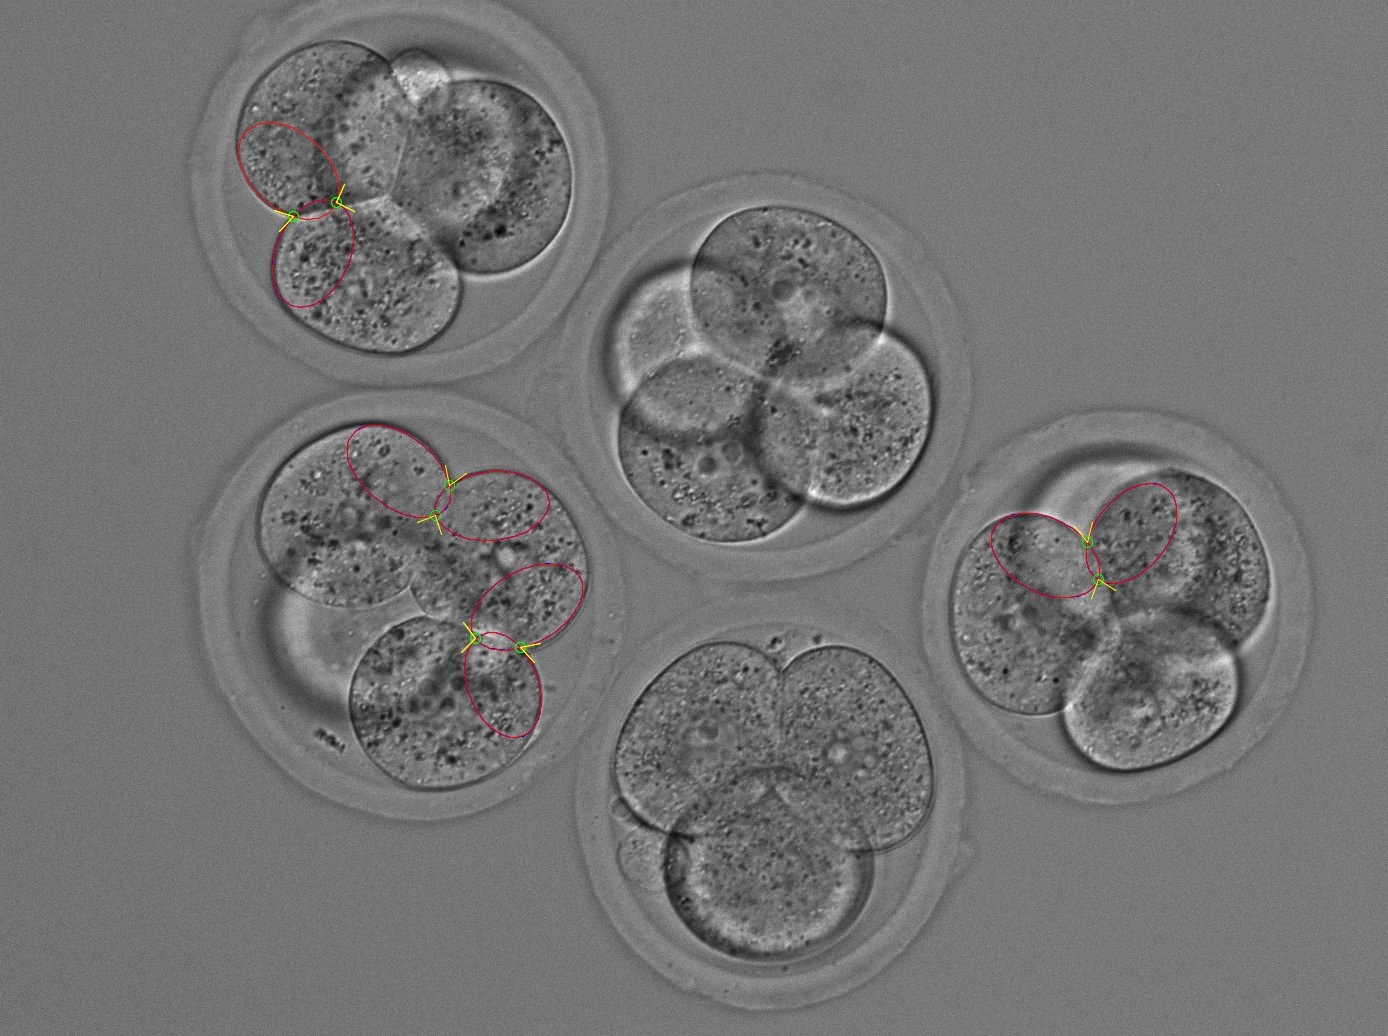
\includegraphics[clip=true,width=1\textwidth]{EmbryoB.jpg}}

}

\frame{\frametitle{ETrack}
\begin{center}
{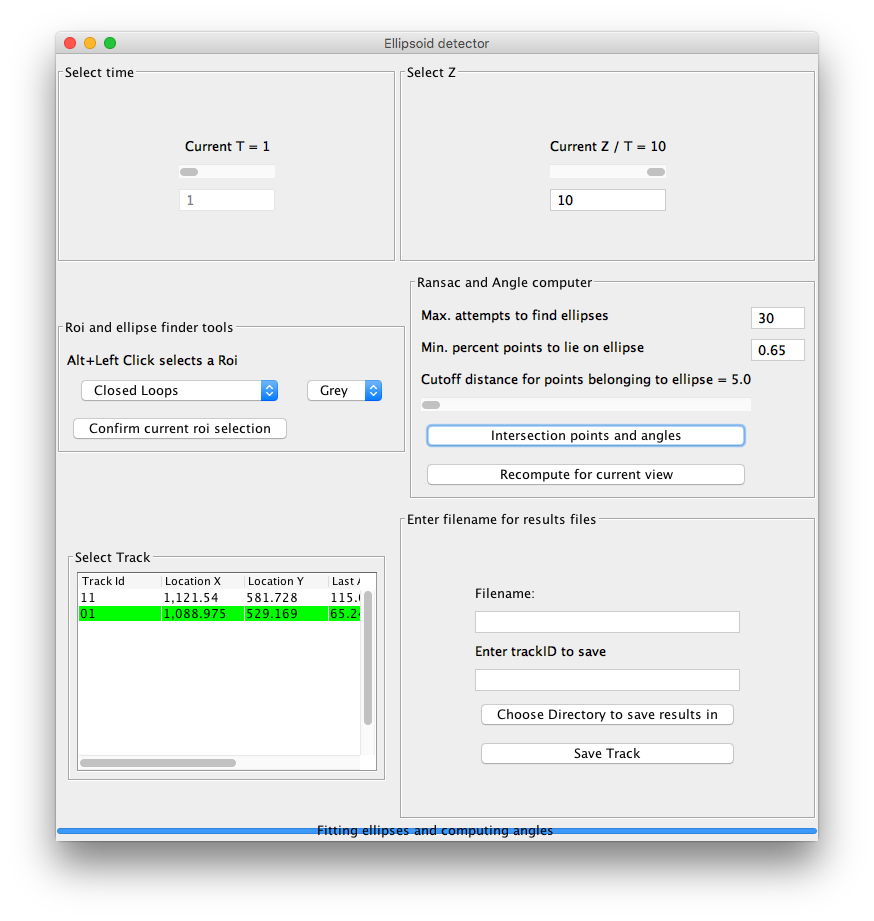
\includegraphics[clip=true,width=0.6\textwidth]{SemiETrack.png}}
\end{center}
}

\frame{\frametitle{Angles}
\begin{columns}
 \begin{column}{0.5\textwidth} 
{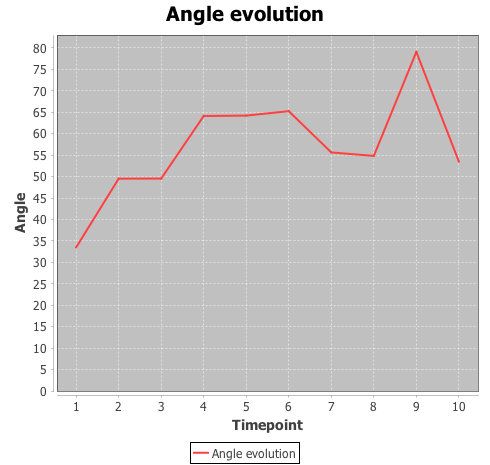
\includegraphics[clip=true,width=1\textwidth]{Angle01.png}}\\
\end{column}
 \begin{column}{0.5\textwidth} 
{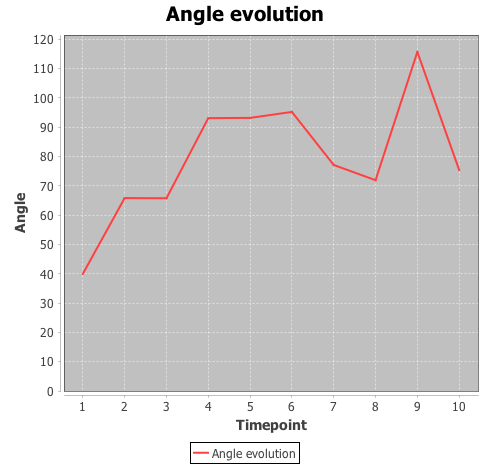
\includegraphics[clip=true,width=1\textwidth]{Angle02.png}}\\
\end{column}
\end{columns}
}
\frame{\frametitle{Random Forest Classifier}

\begin{itemize}
\item How to get Candidate points for ellipse fitting automatically?
\end{itemize}
{\includegraphics[clip=true,width=1\textwidth]{PixelClass.png}}


}
\frame{\frametitle{Take 1}
\begin{center}
\movie[width=1\textwidth, height= 0.5\textwidth]{Click}{Ilastiktake1.mov}
\end{center}
}

\section{Want Perfect Segmentation?}
\subsection{RAF based tool: Ilastik}

\frame{\frametitle{Probability Maps}

\begin{columns}
 \begin{column}{0.5\textwidth} 
 Raw Image
 {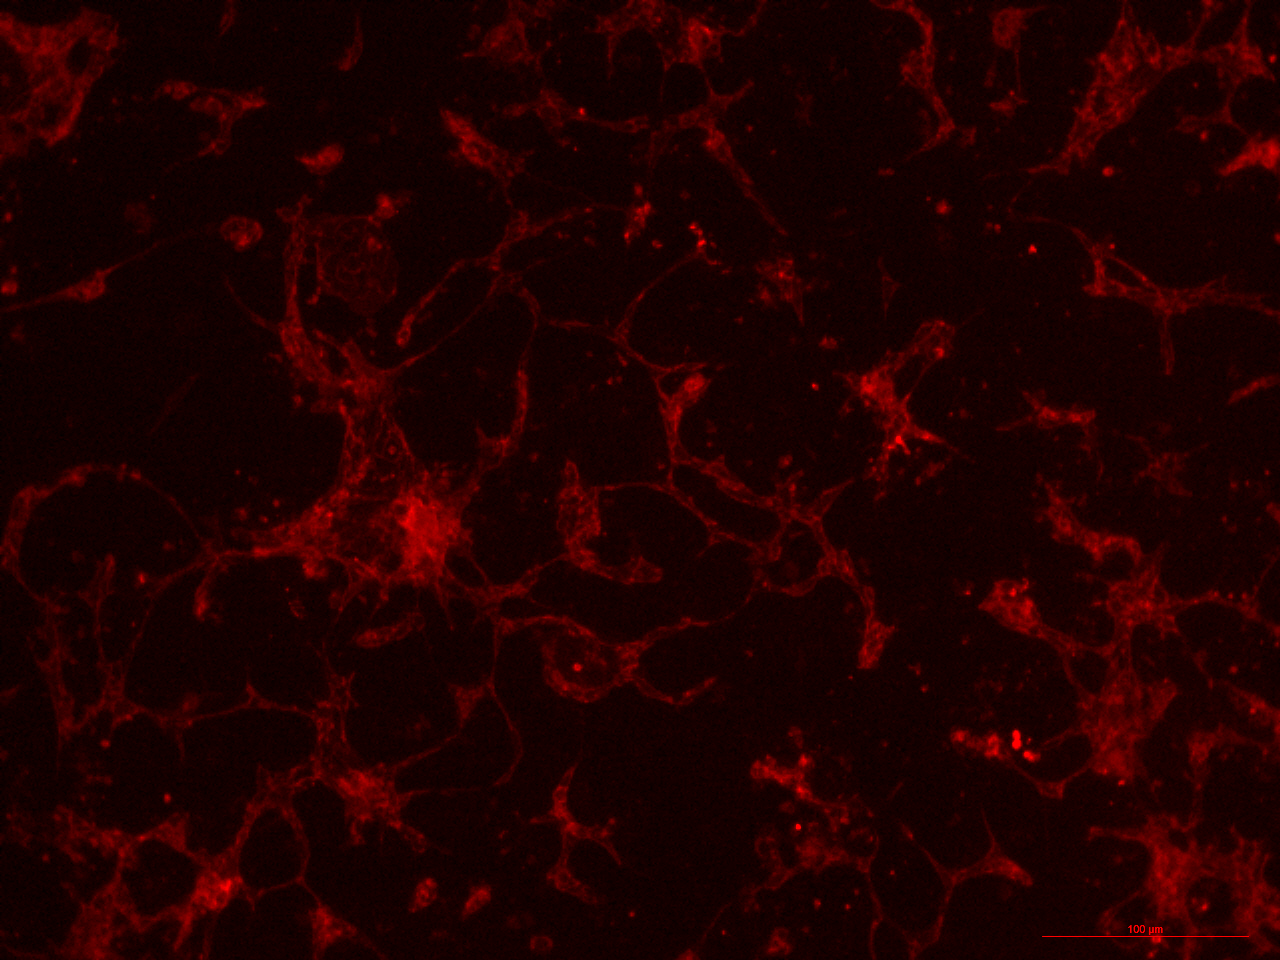
\includegraphics[clip=true,width=1\textwidth]{Unlabelled_Data.png}}\\

\end{column}
 \begin{column}{0.5\textwidth} 
 Tube Probablity Pixels
{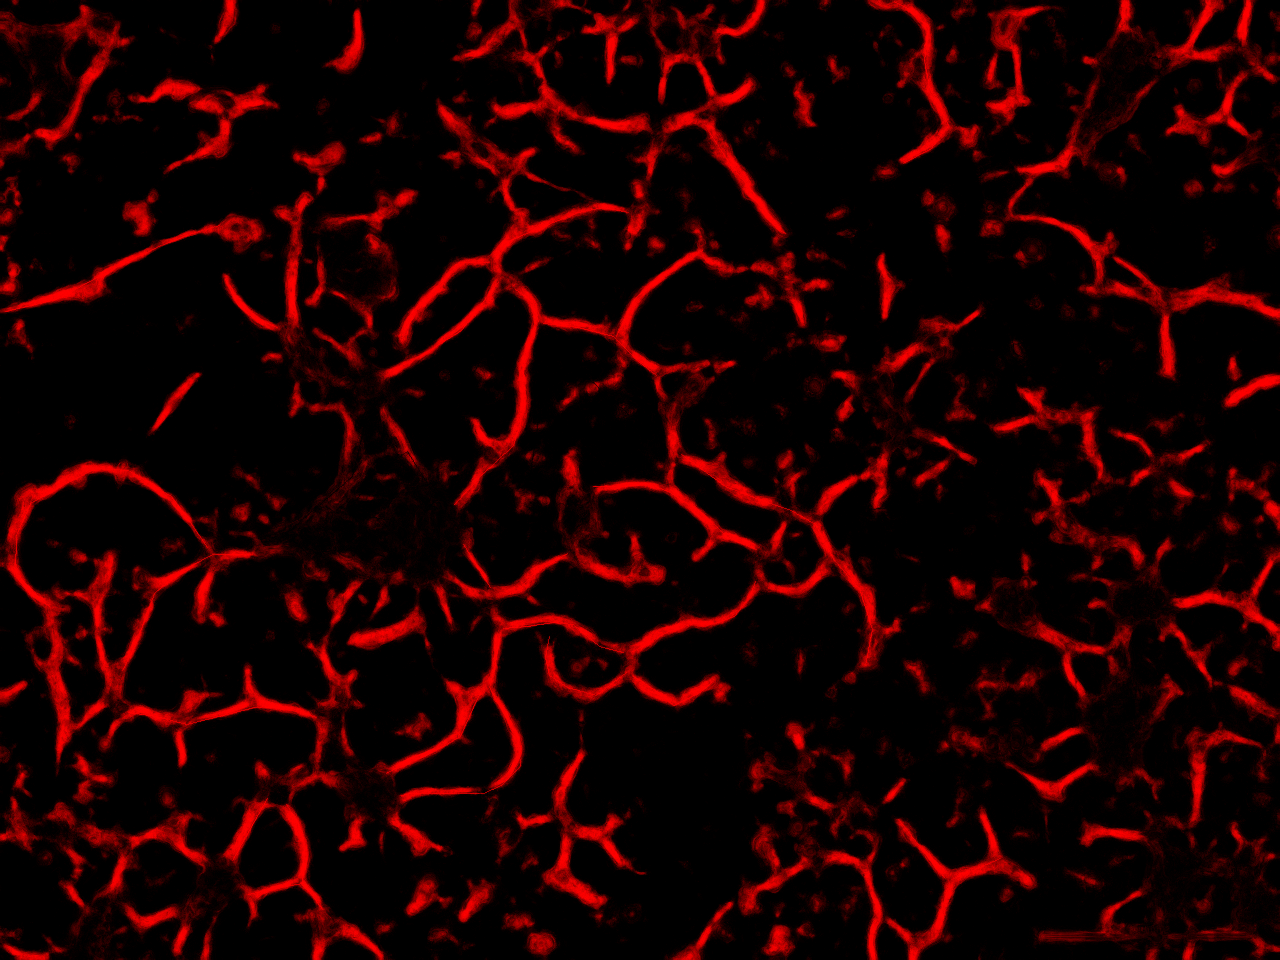
\includegraphics[clip=true,width=1\textwidth]{FinalTubeProbability.png}}\\
\end{column}
\end{columns}
}


\frame{\frametitle{Labelled DataSet Generator}

\begin{center}
{\includegraphics[clip=true,width=1\textwidth]{LabelledDataSetgen.png}}
\end{center}

}

\frame{\frametitle{CoViSTo}

Computer Vision Segmentation tools (CoViSTo).

\begin{columns}
 \begin{column}{0.33\textwidth} 

 {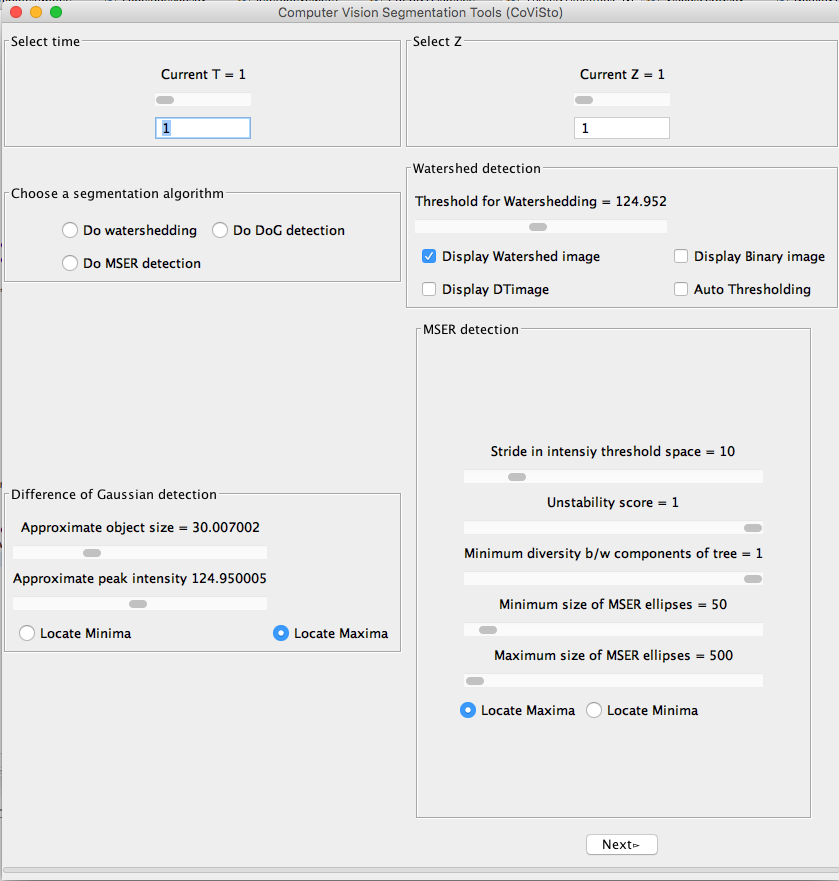
\includegraphics[clip=true,width=1\textwidth]{CoVisTo-panel1.png}}\\

\end{column}
 \begin{column}{0.33\textwidth} 
 
{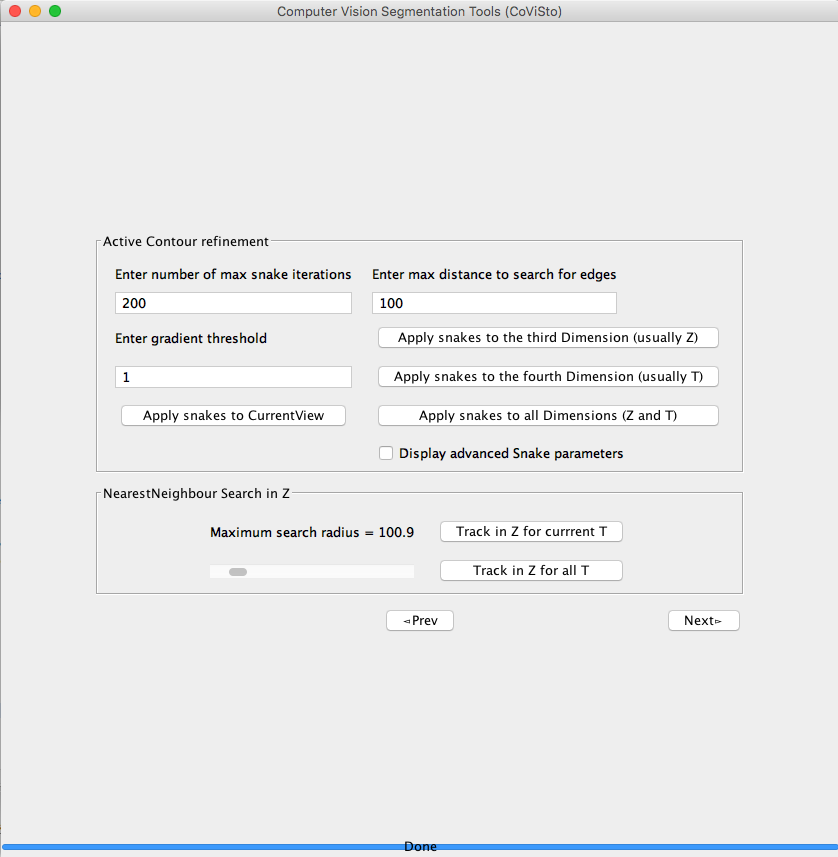
\includegraphics[clip=true,width=1\textwidth]{CoVisTo-panel2.png}}\\
\end{column}
 \begin{column}{0.33\textwidth} 
 
{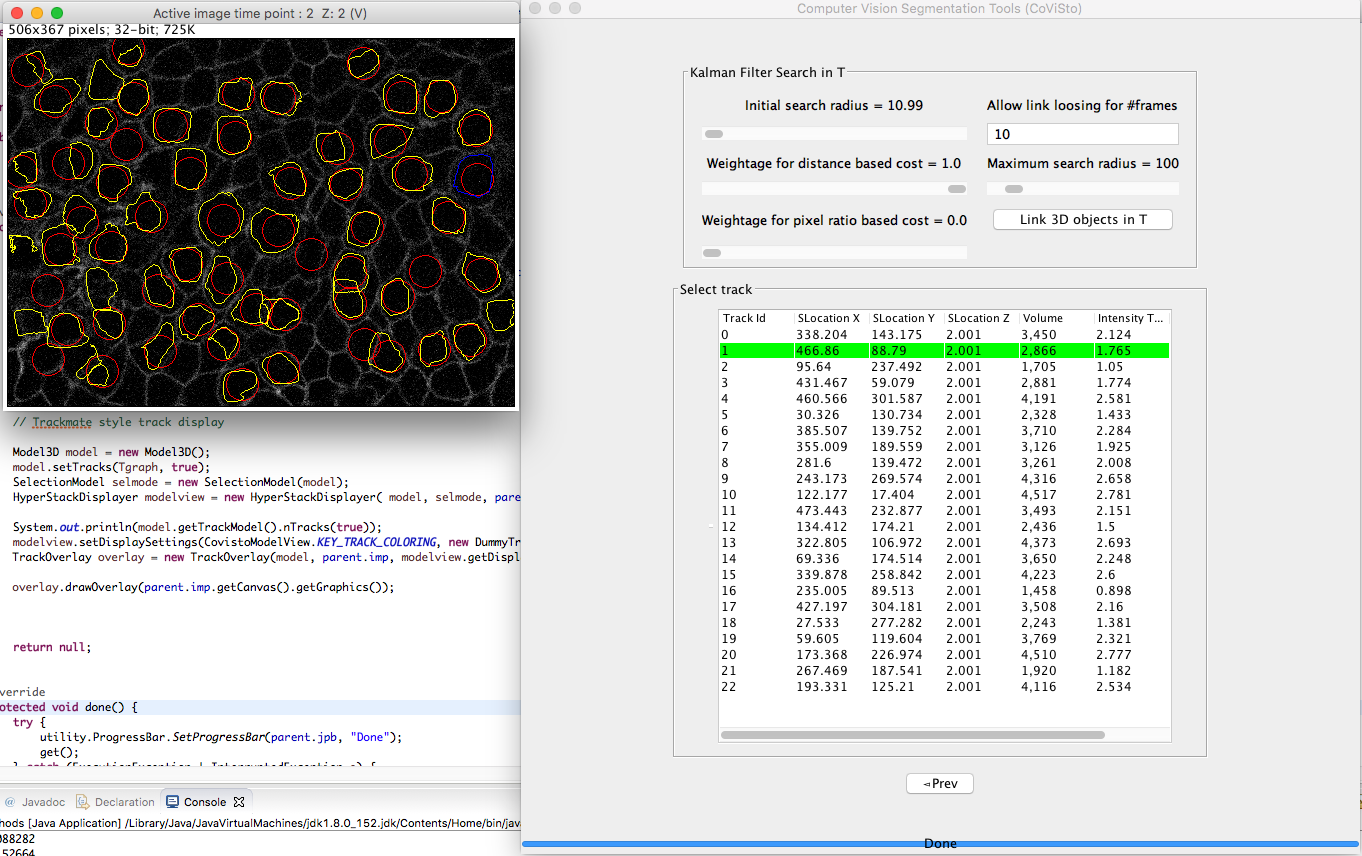
\includegraphics[clip=true,width=1\textwidth]{CoVisTo-panel3.png}}\\
\end{column}
\end{columns}


}
\frame{\frametitle{Job}
\begin{columns}
 \begin{column}{0.5\textwidth} 
{
\includegraphics[clip=true,width=1\textwidth]{job.png}}
\end{column}

 \begin{column}{0.5\textwidth} 
{
\includegraphics[clip=true,width=1\textwidth]{jobsec.png}}
\end{column}
\end{columns}
}
\frame{\frametitle{Conclusions}
Boolean followme = true;

if(followme)\{

https://github.com/kapoorlab

https://twitter.com/EntraCod

\}
\begin{center}
{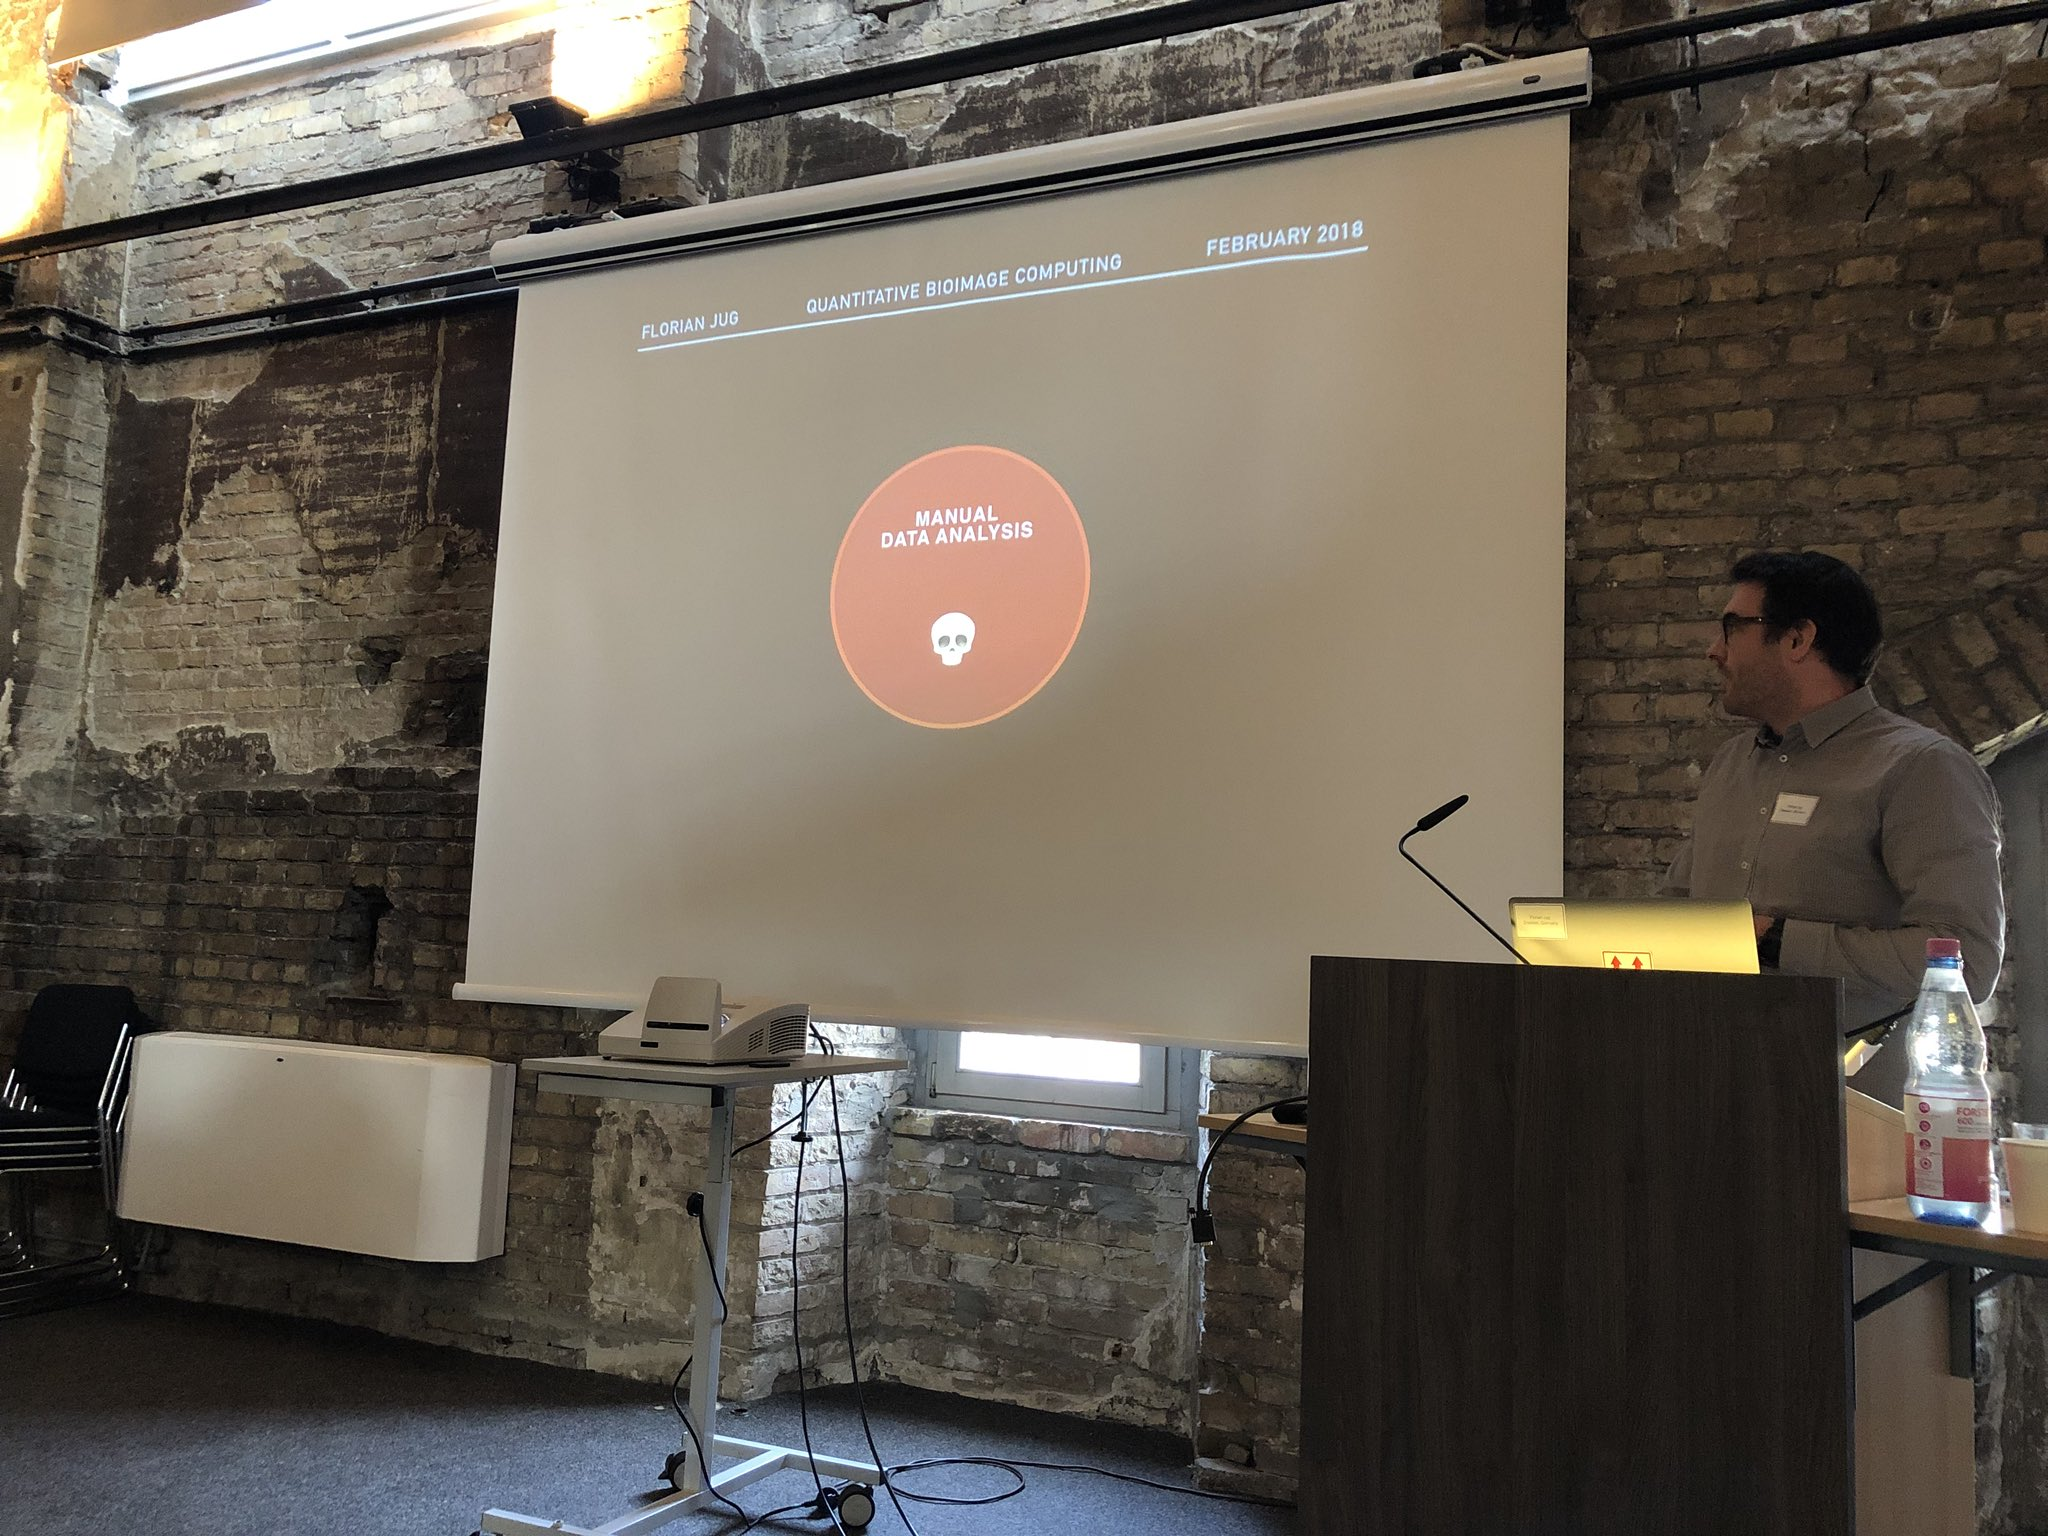
\includegraphics[clip=true,width=0.7\textwidth]{manualdata.jpg}}
\end{center}

}



\end{document}
